\documentclass{article}
\usepackage[letter, margin=1in]{geometry}
\usepackage[utf8]{inputenc}
\usepackage[
    style=authoryear
]{biblatex}
\addbibresource{references.bib}
\usepackage{todonotes}
\usepackage{subcaption}
\usepackage{caption}
\usepackage{graphicx}
\usepackage{hyperref}
\usepackage{float}
\usepackage[framed,numbered,autolinebreaks,useliterate]{mcode}
\hypersetup{
    colorlinks=true,
    linkcolor=blue,
    filecolor=blue,      
    urlcolor=blue,
    citecolor=blue,
    pdftitle={Porad: Structured Light Profilometry for Obstacle Detection and Navigation in Underwater Autonomous Vehicles},
    pdfpagemode=FullScreen,
    pdfauthor={Ari Porad}
}

\newcommand{\code}{\texttt}

\title{Structured Light Profilometry for Obstacle Detection and Navigation in Underwater Autonomous Vehicles}
\author{Ari Porad\\RoboLab, Olin College of Engineering}
\date{Spring 2021}

\begin{document}

\maketitle

\begin{abstract}
    \label{abstract}
    I researched the use of structured light profilometry for underwater autonomous navigation and obstacle detection. The project progressed to the prototype phase, where I built a desktop test bed that contained a line laser, a camera (with a bandpass filter), and a Raspberry Pi for computation. The system was capable of successfully detecting the position of the laser beam within the camera frame, but more development is needed to properly derive physical object positions, and to differentiate between multiple objects.
\end{abstract}

\begin{center}
    \textbf{\small{Source Code}}\\
    \smallskip
    All source code for this project can be found at: \hyperlink{https://github.com/ariporad/robofish-SP21}{https://github.com/ariporad/robofish-SP21}.
\end{center}

\section{Introduction} \label{sec:intro}

The Olin RoboLab is currently engaged in a multi-year effort to develop a versatile, efficient, and bio-realistic autonomous robotic fish for littoral surveying. A significant area of research for this project is the development of a system for navigation and obstacle avoidance. Our target underwater terrain is frequently dark, rendering traditional computer vision systems inoperable. Any form of broad active illumination to supplement a traditional computer vision system is infeasible due to power limitations.

Structured light profilometry offers a promising alternative to these traditional vision systems. By using a focused laser beam, the power requirements are drastically reduced without sacrificing illumination distance. While a line laser is only capable of calculating depth data in one dimension (therefore producing a two-dimensional result), the forward motion of the fish can be used to recreate the third dimension over time. This technology has a wide-ranging array of possible uses, from underwater surveying to submarine navigation.

Structured light is often used in highly-controlled factory contexts to measure surfaces without touching them (\cite{salvi_state_2010, tsai_development_2005}). It was also previously researched by students in the Olin RoboLab on a previous incarnation of the robot fish project (\cite{barrett_applying_2018}). However, it has to the best of the author's knowledge never been perfected in an underwater, uncontrolled context. This report details my research into this topic over the course of the Spring 2021 semester. While much progress was made, far more is yet to be done to continue validating this promising technology.

\section{Methods} \label{sec:methods}

\subsection{Software} \label{sec:methods:software}

\subsubsection{Platform} \label{sec:methods:software:platform}

I used a Raspberry Pi 4 Model B as the system's controller. The Pi 4 is affordable, powerful, and easy to use. It has a robust camera ecosystem (see \ref{sec:methods:hardware:optics-camera}), a mechanism for interfacing with electronics directly (via \href{https://www.raspberrypi.org/documentation/usage/gpio/}{GPIO pins}), and is generally well-suited to robotic experimentation.

All code for this project was written in MATLAB. MATLAB is well suited to rapid prototyping, on account of being rather flexible and having a large set of (mostly) easy-to-use and turn-key toolboxes. For example, I was able to use MATLAB's built in camera calibrator to correct for lens distortion in less than an hour. However, MATLAB is generally poorly suited to writing large amounts of scalable or performant software (it's very much a mechanical engineer's programming language).\footnote{I had a brief foray into using C++ and OpenCV instead of MATLAB, which did indeed produce better code at the expense of having a much lower development velocity. I ultimately returned to MATLAB in the name of efficiency.}

Additionally, MATLAB has a \href{https://www.mathworks.com/help/supportpkg/raspberrypiio/index.html}{built-in Raspberry Pi integration}. With it, all code runs on a separate laptop and simply communicates with the Pi over Wi-Fi. This configuration prevents the Pi's limited processing power from being a bottleneck, and makes development drastically easier (no need to write code over SSH, or synchronize files, etc.).
    
\subsection{Hardware} \label{sec:methods:hardware}

\subsubsection{Optics: Camera} \label{sec:methods:hardware:optics-camera}

For the system's main camera, I used a Raspberry Pi \href{https://www.raspberrypi.org/products/raspberry-pi-high-quality-camera/}{High Quality Camera}. I chose the HQ Camera for its simple integration with the Raspberry Pi (and with MATLAB) and it's flexibility: I anticipated wanting to experiment with various lenses, and so having a removable lens was enticing. Additionally, having a standard-size removable lens opened the possibility of using a \hyperlink{https://www.rmaelectronics.com/midwest-optical-bn535/}{C-Mount bandpass filter} (see below), which would have been extremely clean and convenient. However, I wasn't able to successfully source a C-Mount lens---nor did I need to use different lenses---so the simplicity of a standard Raspberry Pi \hyperlink{https://www.raspberrypi.org/products/camera-module-v2/}{Camera Module} would have been preferable.

I used a standard Raspberry Pi HQ Camera \hyperlink{https://www.sparkfun.com/products/16762}{6mm Wide Angle CS-mount lens}. In front of the lens was a \hyperlink{https://www.rmaelectronics.com/midwest-optical-bn535/}{535nm bandpass filter}\footnote{This is the same model I had hoped to get in a C-Mount configuration, in a different size.}, which filtered out all light other than the laser light (or other light the same color). This resulted in the camera's image being essentially 1 bit---if there was any light at all, then it had to be the laser(see \ref{sec:methods:hardware:optics-camera}). In practice, this was decent but imperfect because the laser was bright enough that it would also illuminate other things (especially the floor, see \autoref{fig:image:raw}), so there still needed to be some filtering of laser vs. not laser in software.

\subsubsection{Optics: Laser} \label{sec:methods:hardware:optics-laser}

A \hyperlink{https://smile.amazon.com/Cutting-Locator-Positioning-18x75mm-Heatsink/dp/B07B9W6M6M}{relatively-inexpensive line laser} was used. While this particular part was easy to get started with, its circular body made it difficult to mount precisely (this resulted in some issues with the laser beam not being perfectly horizontal, which made processing more complicated---see \ref{sec:results:filtering-laser-detection}). Additionally, it was far brighter than required for desktop testing, which possibly contributed to the aforementioned light bleed.\footnote{It's possible this wouldn't be a concern when testing the system underwater (ie. without a floor), but the necessity of desktop testing makes the issue worth addressing irregardless.} It also wasn't eye safe, which made testing procedures substantially more cumbersome (see \ref{sec:methods:testing}).

\subsubsection{Testbed} \label{sec:methods:hardware:testbed}

I built a 3D-printed testbed, which held the laser and camera at a precise angle (along with a the Raspberry Pi itself). The laser was held in place by a wood screw at the manufacturer's recommendation\footnote{I know, I know, using a wood screw to pin a cylinder in place is bad.}. The Pi and Camera were intended to be held in place by screws, but due to tolerance errors had to be held in place with tape. The filter was pinned in place by the mount and the camera.

\begin{figure} [!h]

	\centering
    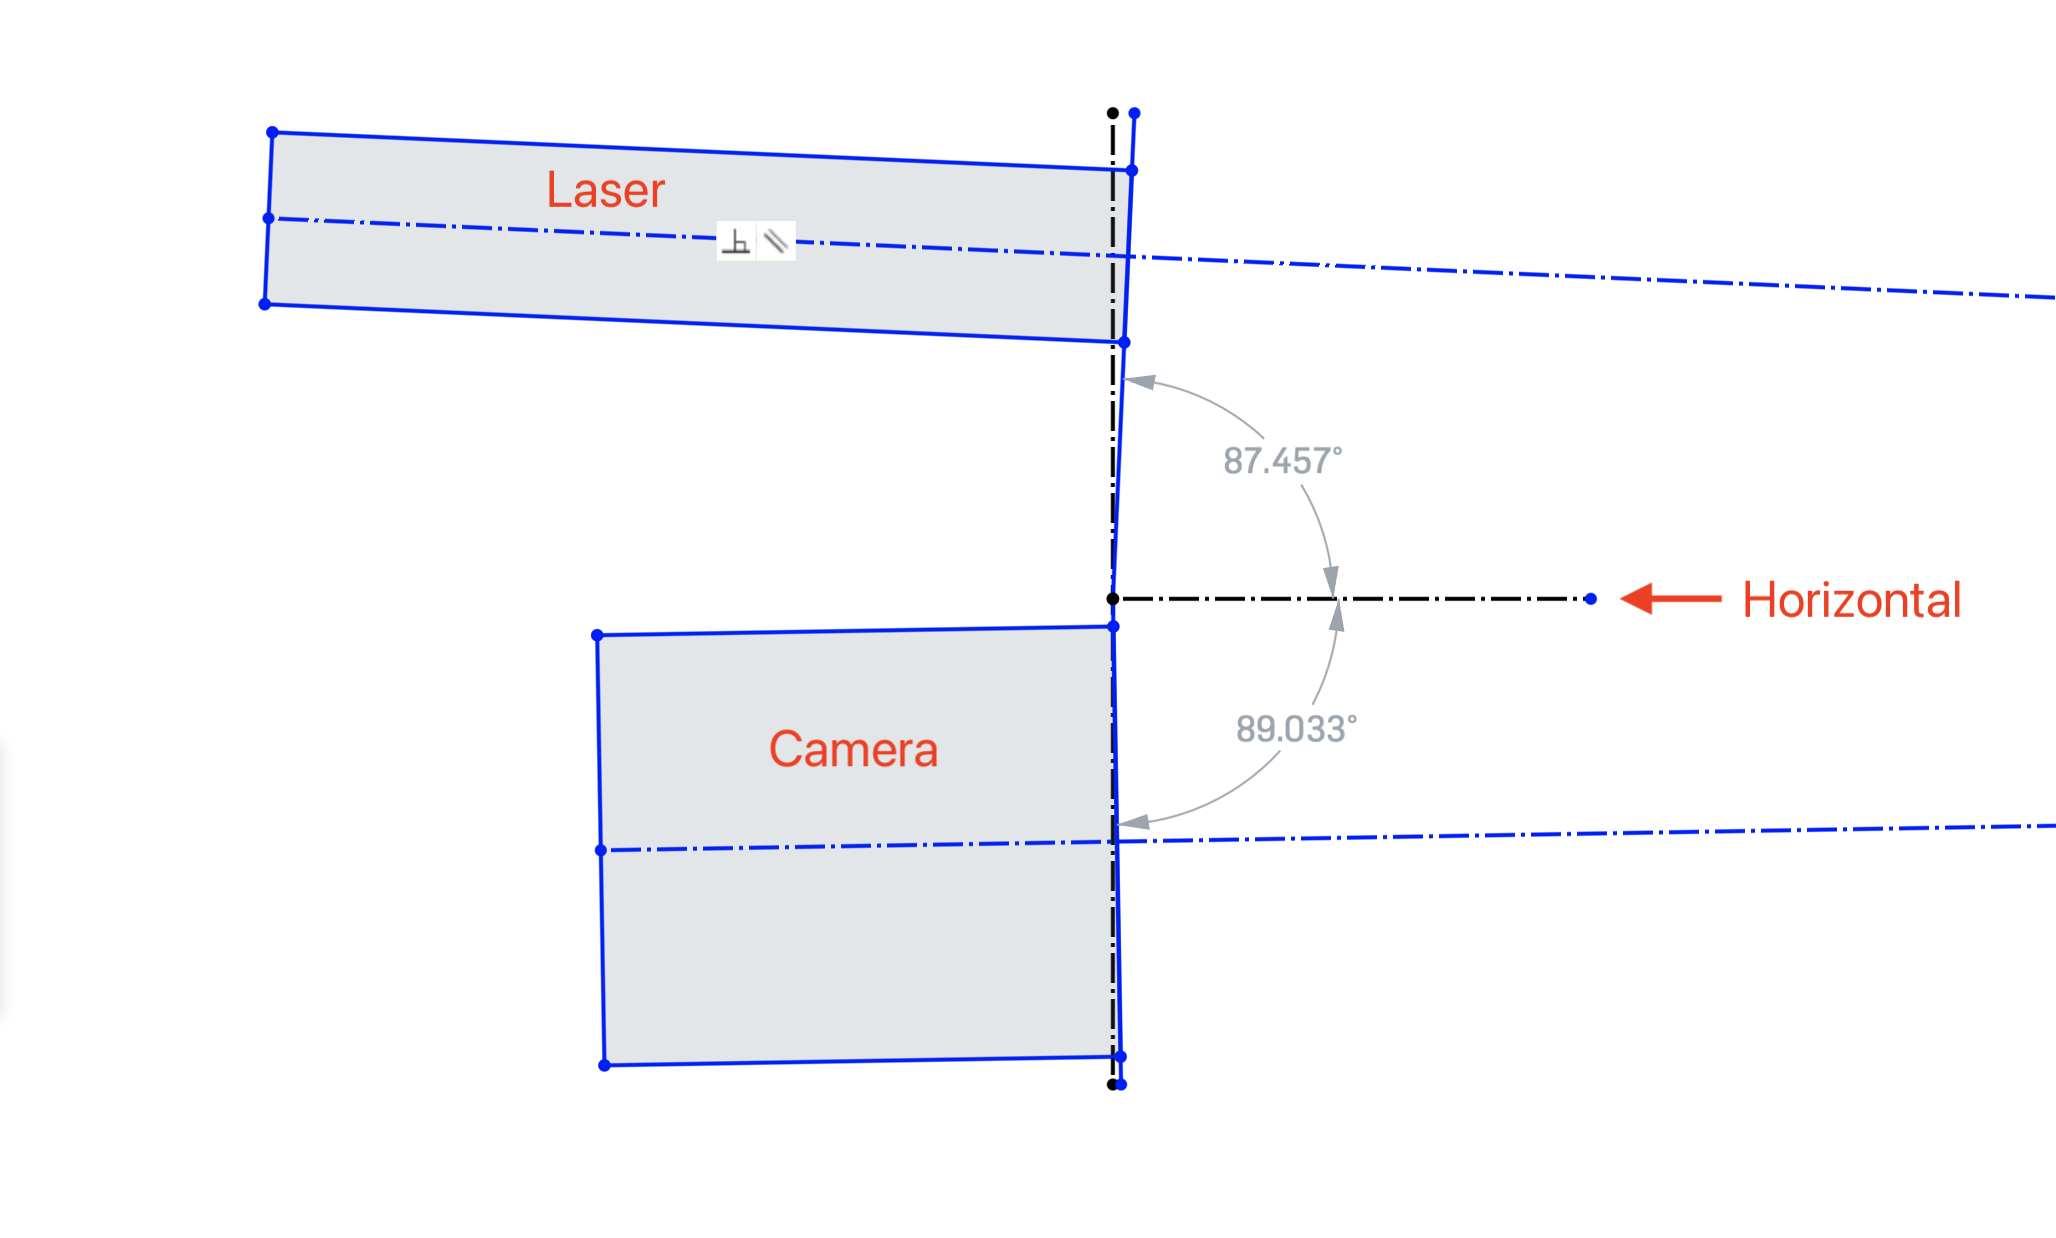
\includegraphics[width=0.8\linewidth]{laser-geometry.png}
	
	\caption{\smaller{CAD rendering of testbed geometry, showing the precise angles of the laser and the camera. No attempt was made to quantify the precision or tolerance of the 3D printer as it pertains to these angles. Blue lines extending to the right represent the center of the camera's view and the center of the laser beam, and intersect at 1 meter (not shown).}}
	
	\label{fig:testbed-geometry}
\end{figure}

\begin{figure} [!h]
	\centering
    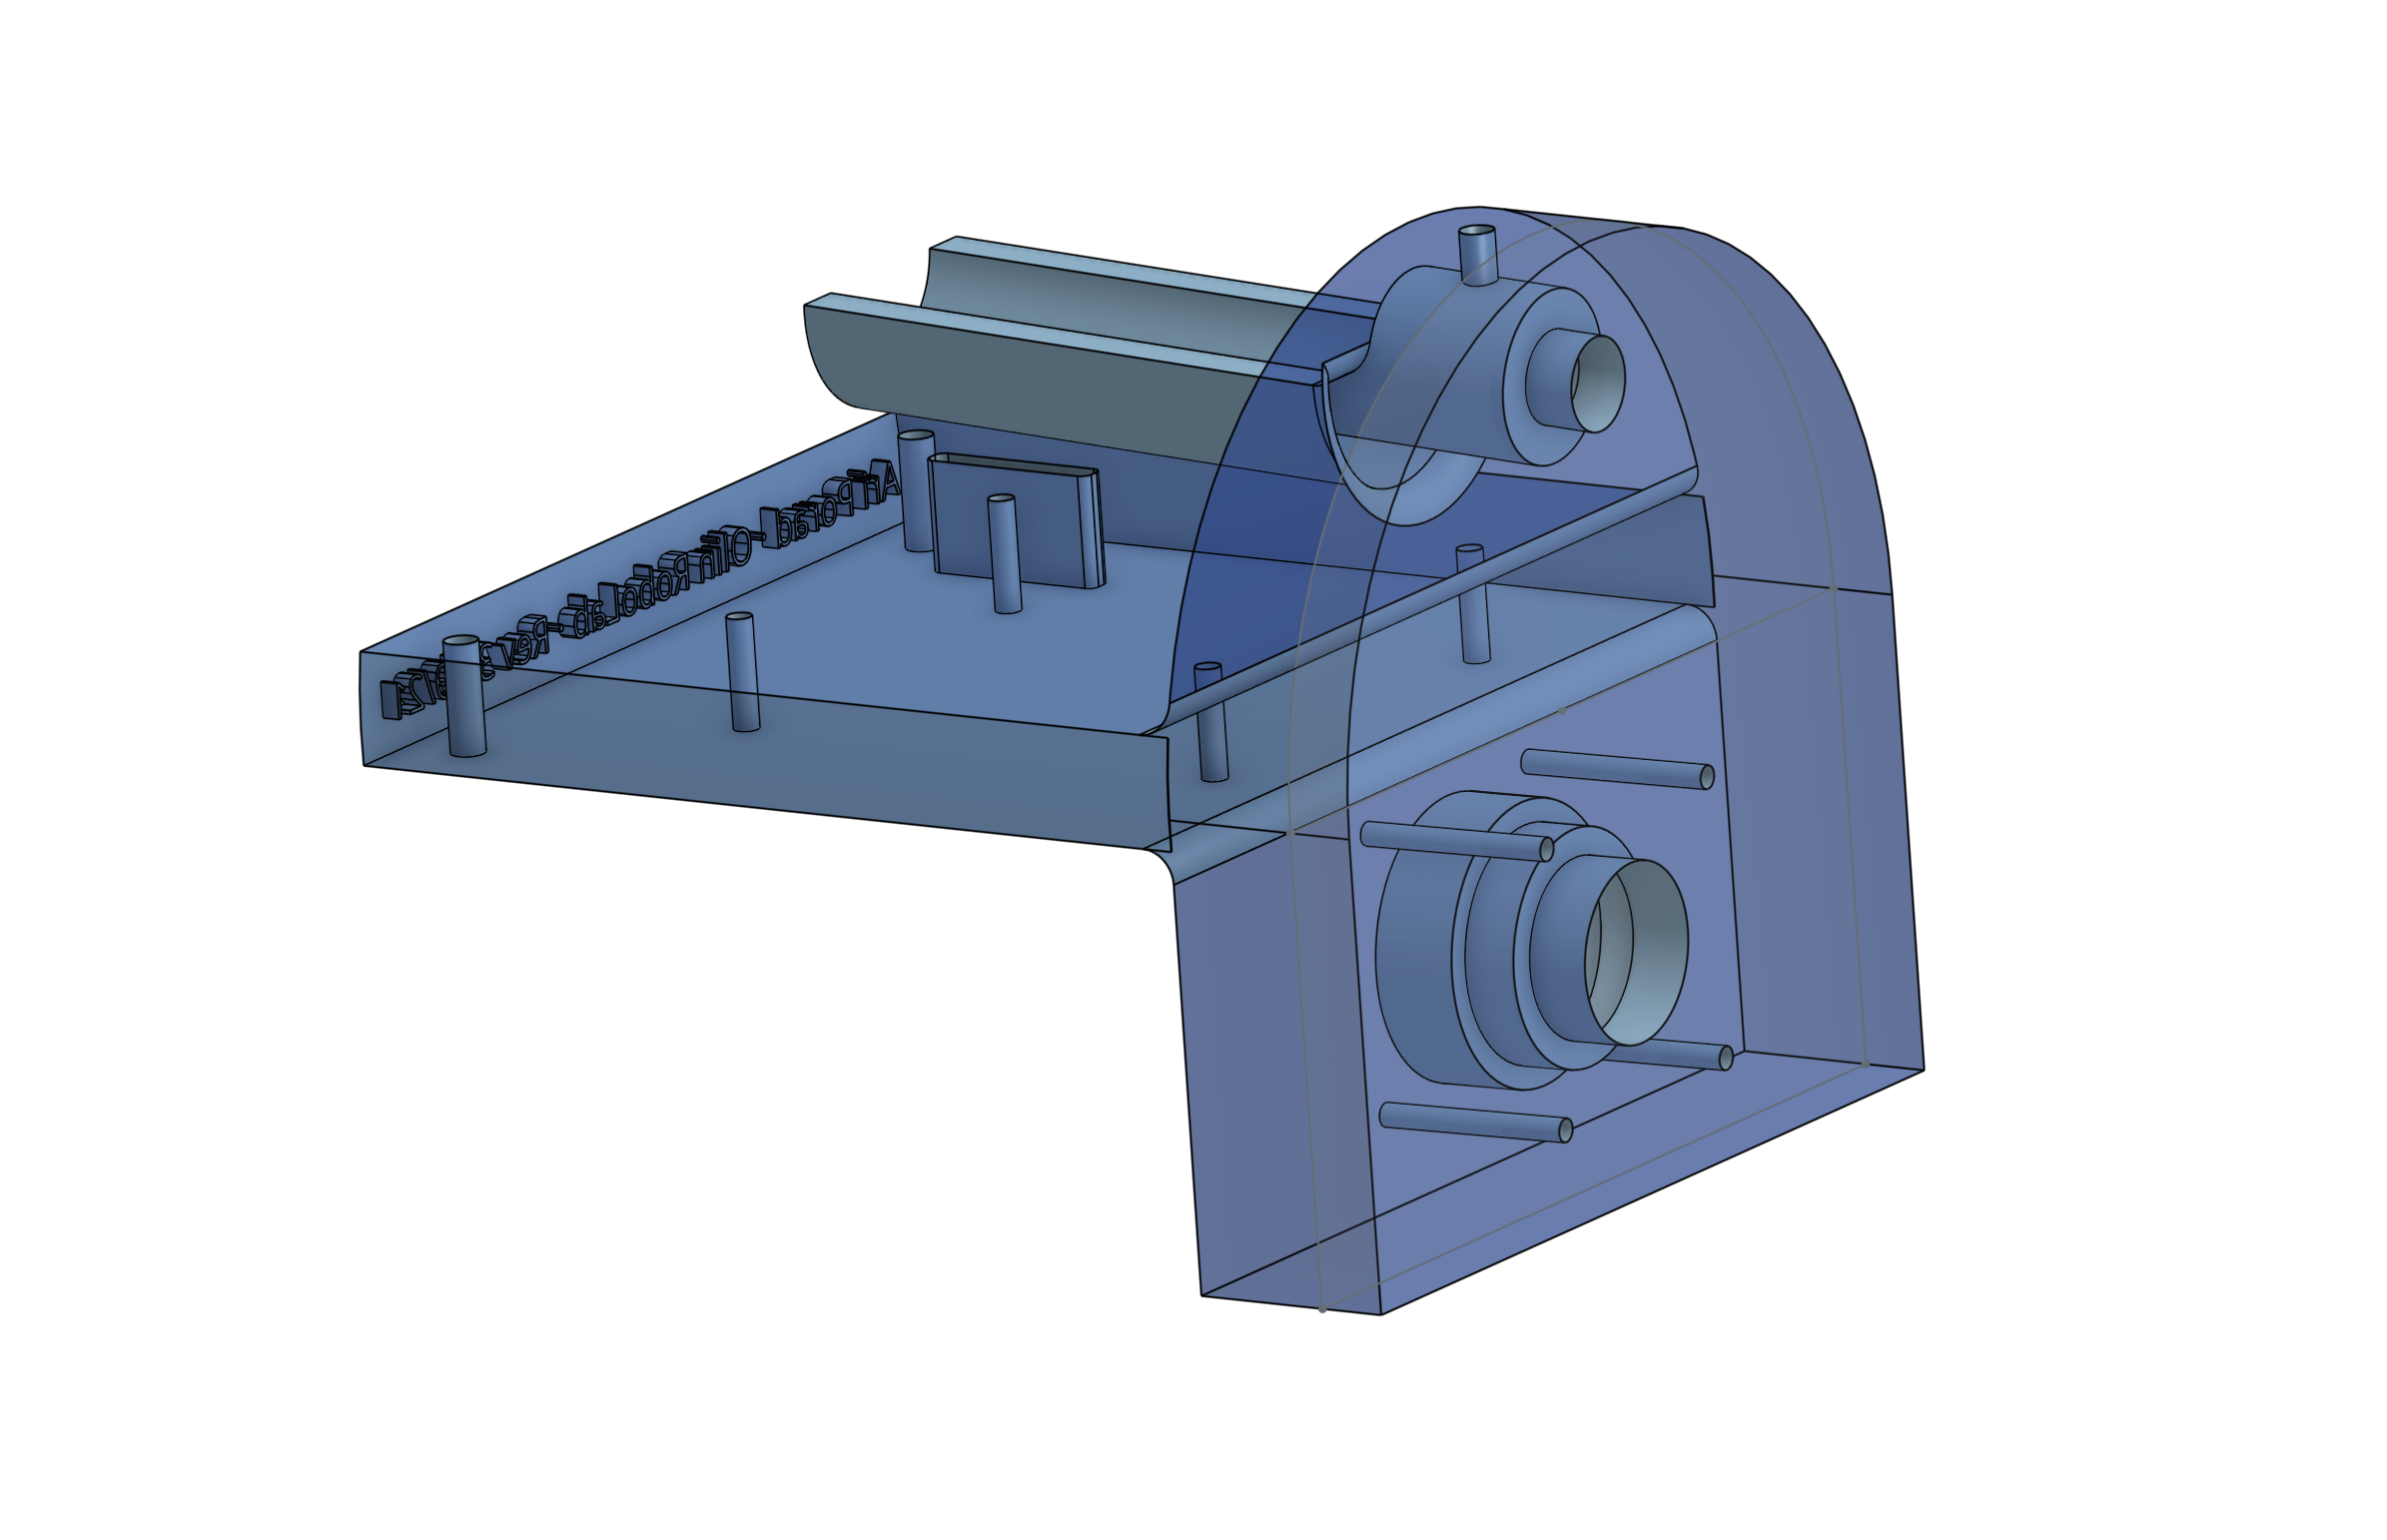
\includegraphics[width=0.65\linewidth]{testbed-transparent.png}
	
	\caption{\smaller{Transparent CAD rendering of the testbed, showing its internal geometry. Camera, Laser, Pi, and screws are not shown.}}
	
	\label{fig:testbed-transparent}
\end{figure}

\begin{figure} [!h]

	\centering
	
	\begin{subfigure}{.5\textwidth}
	    \centering
    	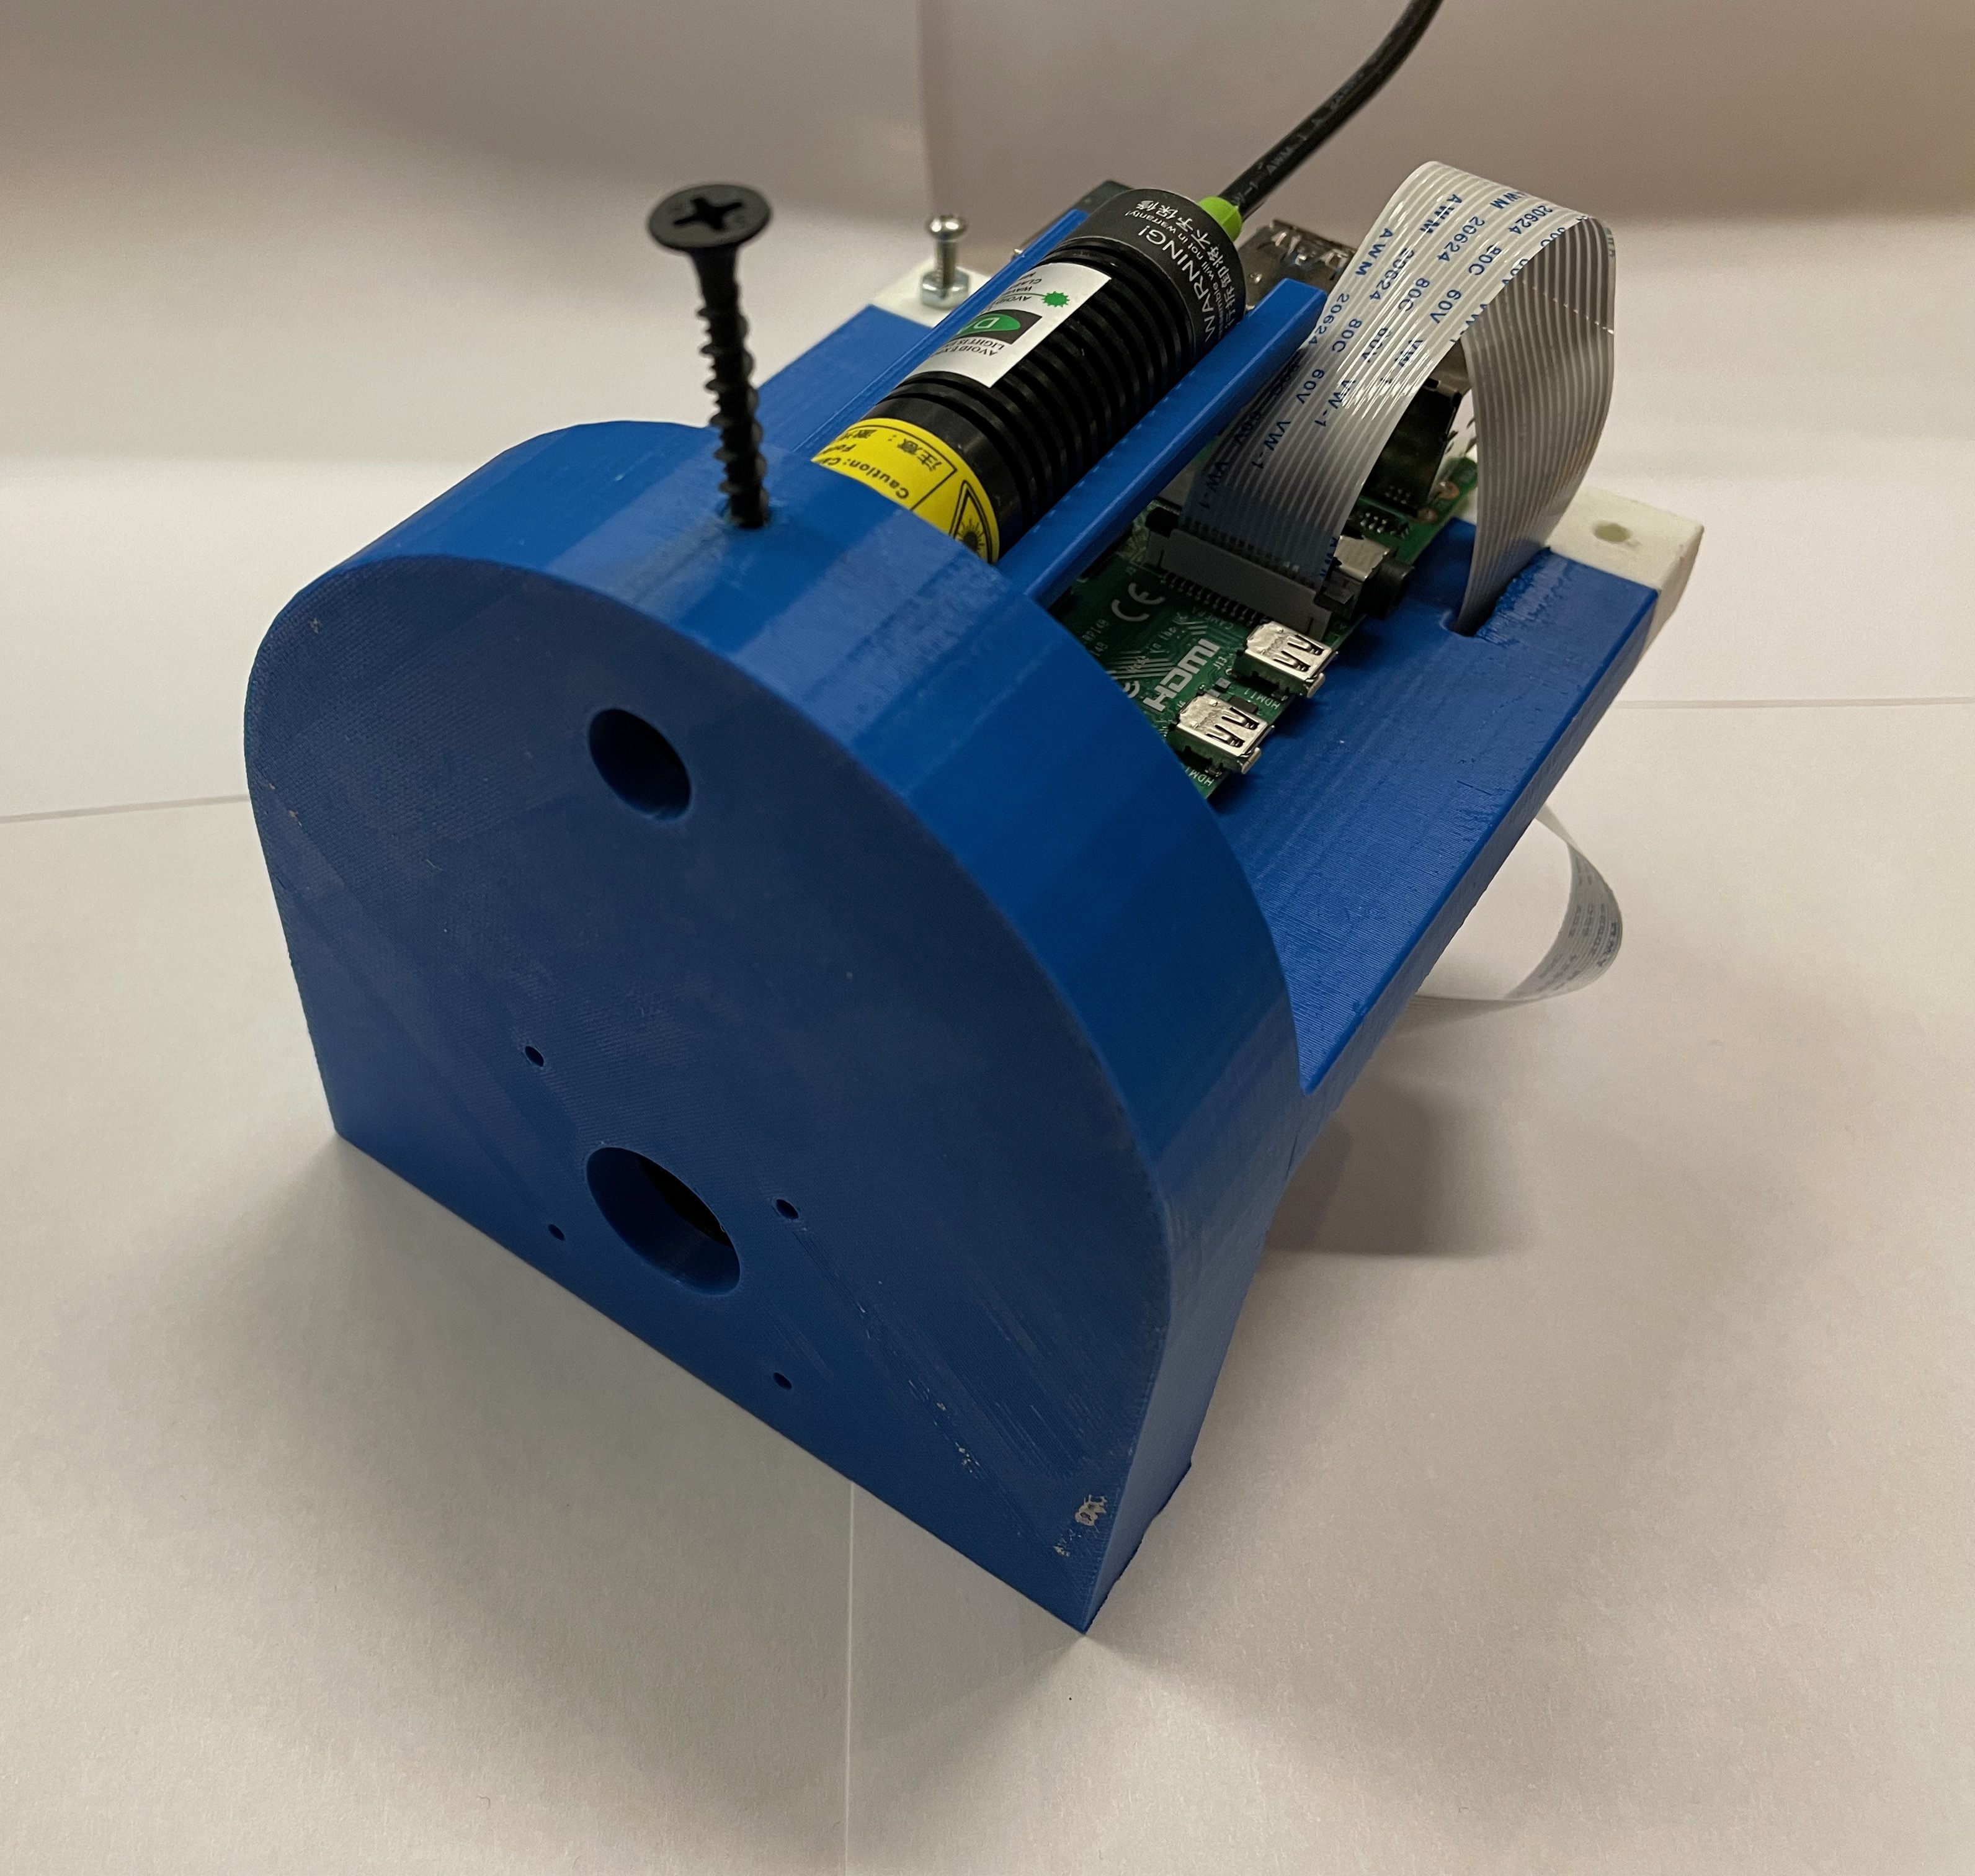
\includegraphics[width=0.8\linewidth]{testbed-front.jpeg}
    	\caption{Front}
    	\label{fig:testbed-printed:front}
    \end{subfigure}% <-- this comment is important to prevent a space
	\begin{subfigure}{.5\textwidth}
	    \centering
    	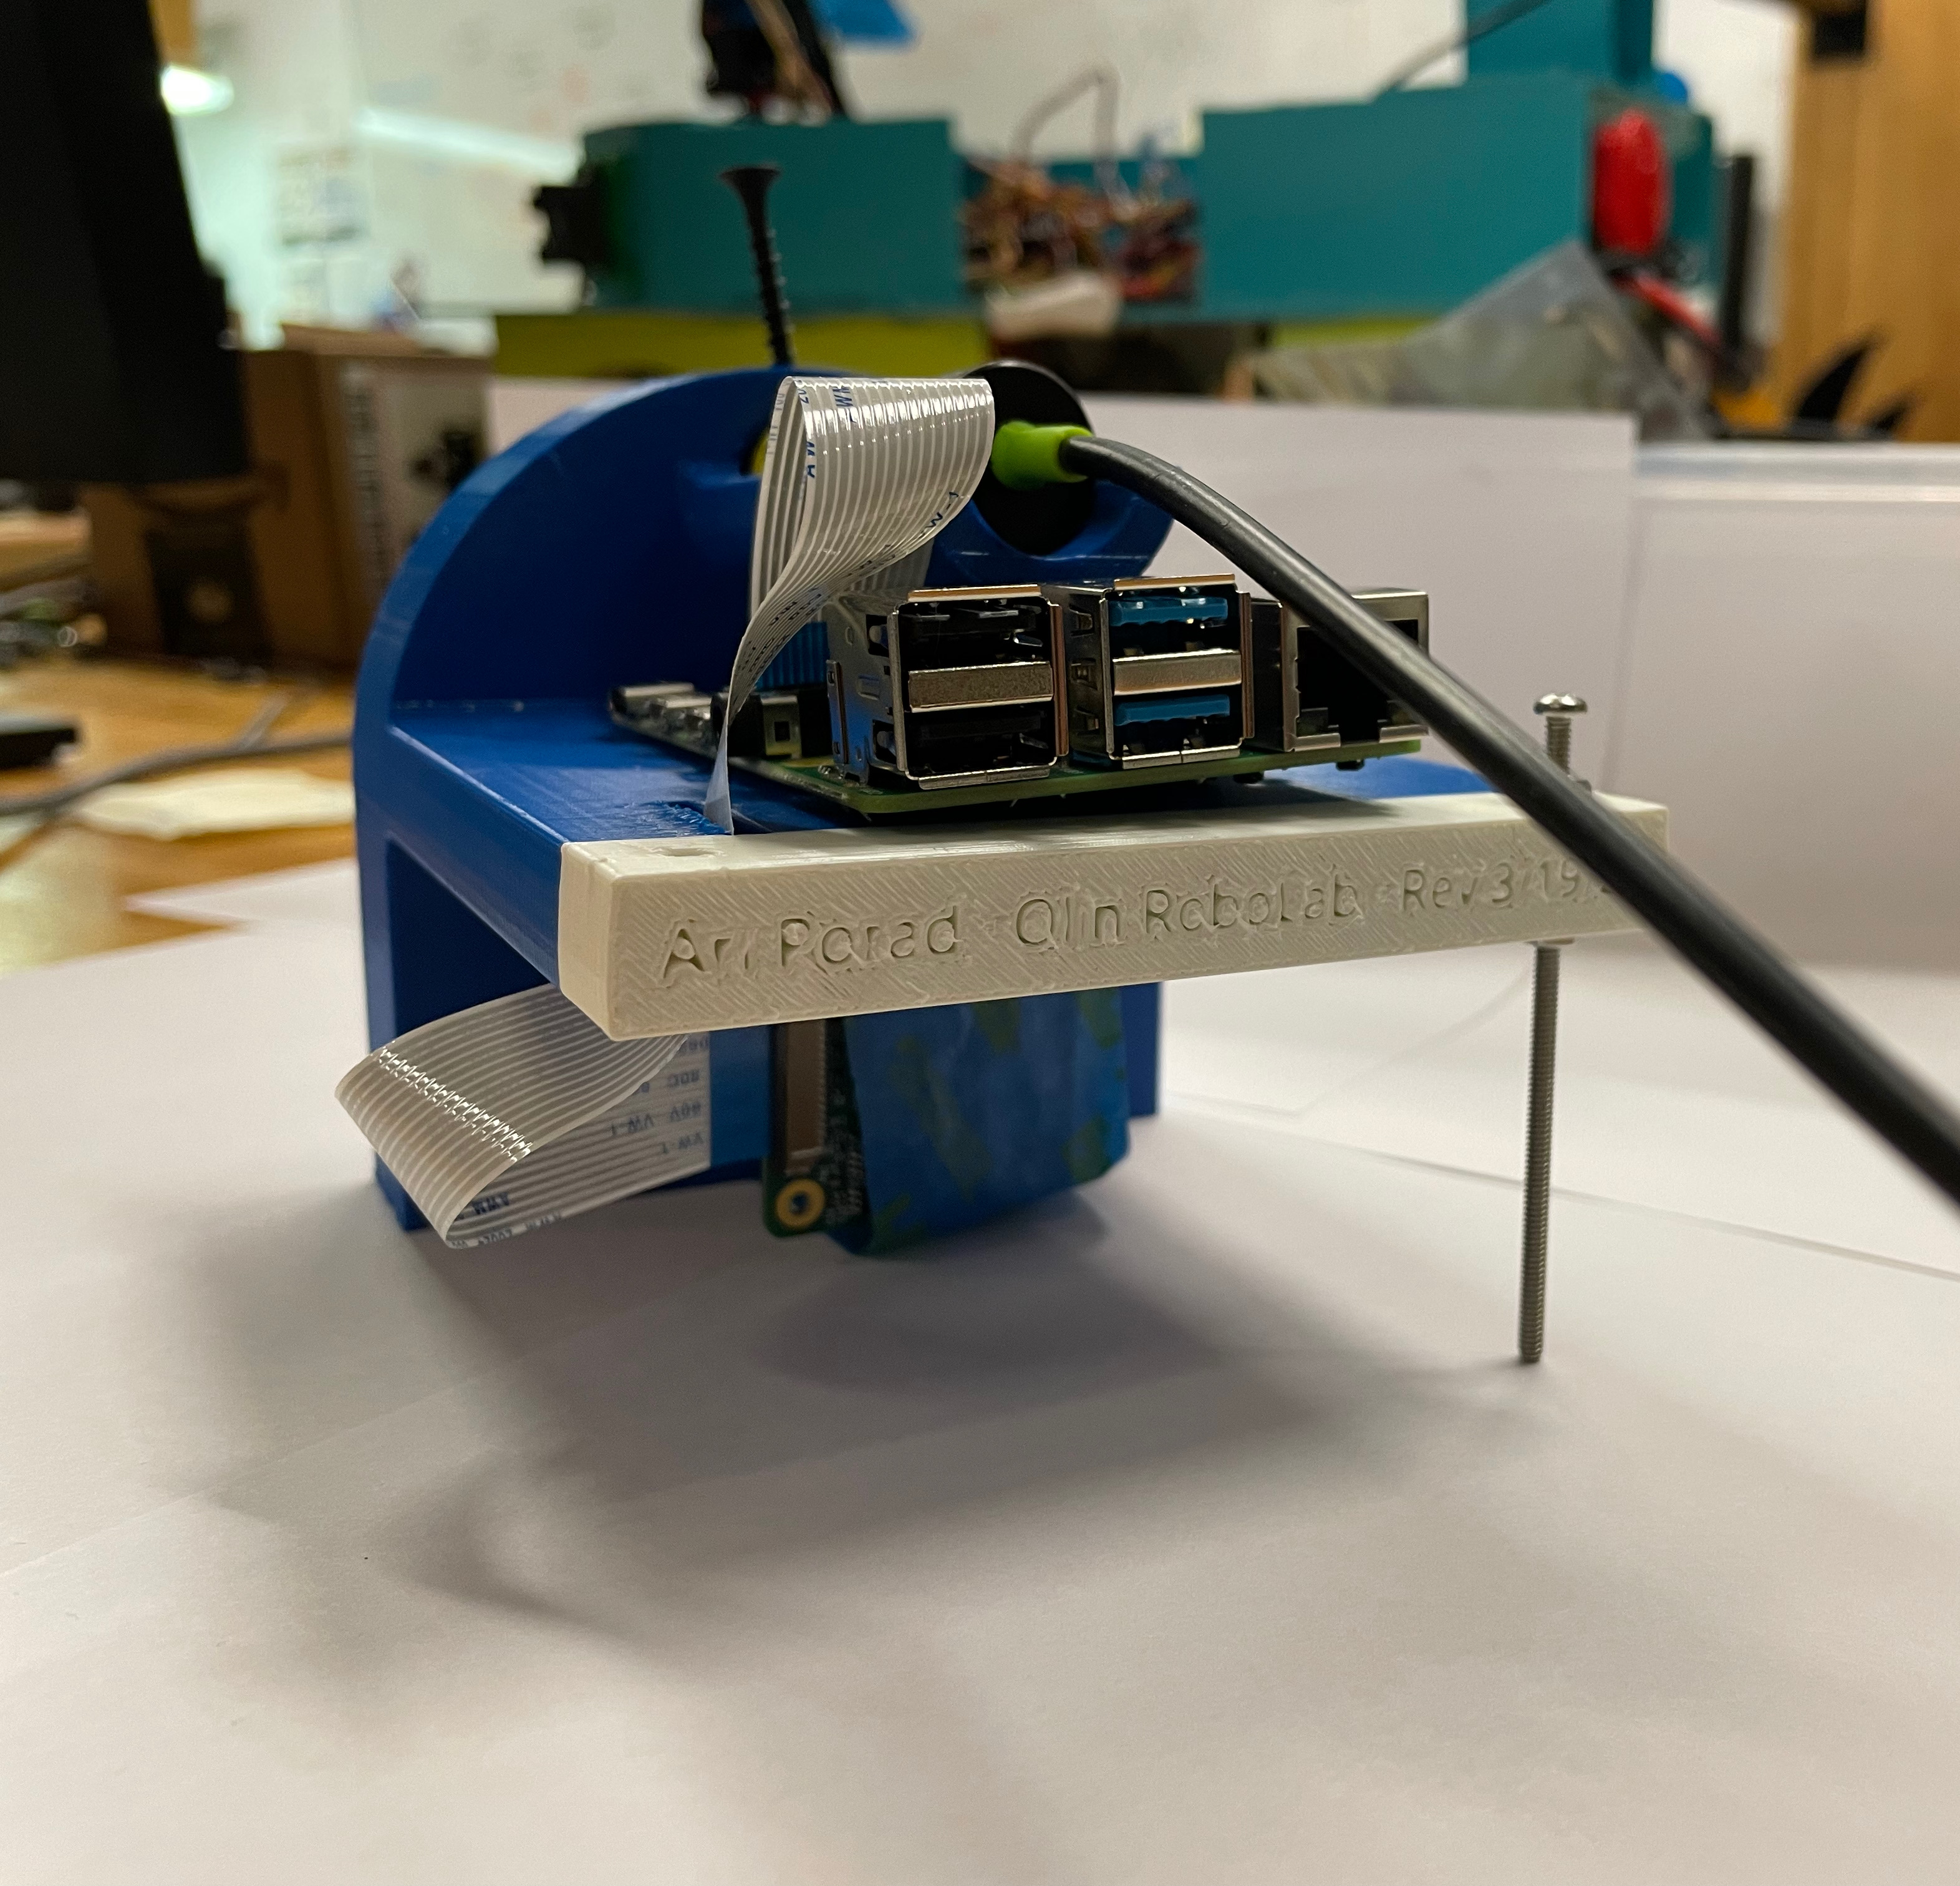
\includegraphics[width=0.8\linewidth]{testbed-back.jpeg}
    	\caption{Back}
    	\label{fig:testbed-printed:back}
    \end{subfigure}
	
	\caption{\smaller{3D-printed testbed prototype. White section is due to running out of filament. The screw in the back-right was to hold up the Pi plate---printing a foot would have required significant amounts of support.}}
	
	\label{fig:testbed-printed}
\end{figure}

\subsection{Testing} \label{sec:methods:testing}

Because the laser I used wasn't eye safe\footnote{While I had appropriate eye protection, it was infeasible to provide adequate protection to everyone in the RoboLab.}, all testing was conducted in an isolated environment---affectionately referred to as the \textit{Laser Cave}.\footnote{Naming Credit: Esme Abbot, 2021} The Laser Cave was constructed by duct-taping cardboard around the feet of a table, ensuring that it was appropriately and fully sealed. The Laser Cave was also outfitted with a means of measuring the distance between the prototype and the target, and with a power supply.

\begin{figure} [!h]

	\centering
	
	\begin{subfigure}{.5\textwidth}
	    \centering
    	\includegraphics[width=0.8\linewidth]{laser-cave-outside.jpeg}
    	\caption{Outside}
    	\label{fig:laser-cave:outside}
    \end{subfigure}% <-- this comment is important to prevent a space
	\begin{subfigure}{.5\textwidth}
	    \centering
    	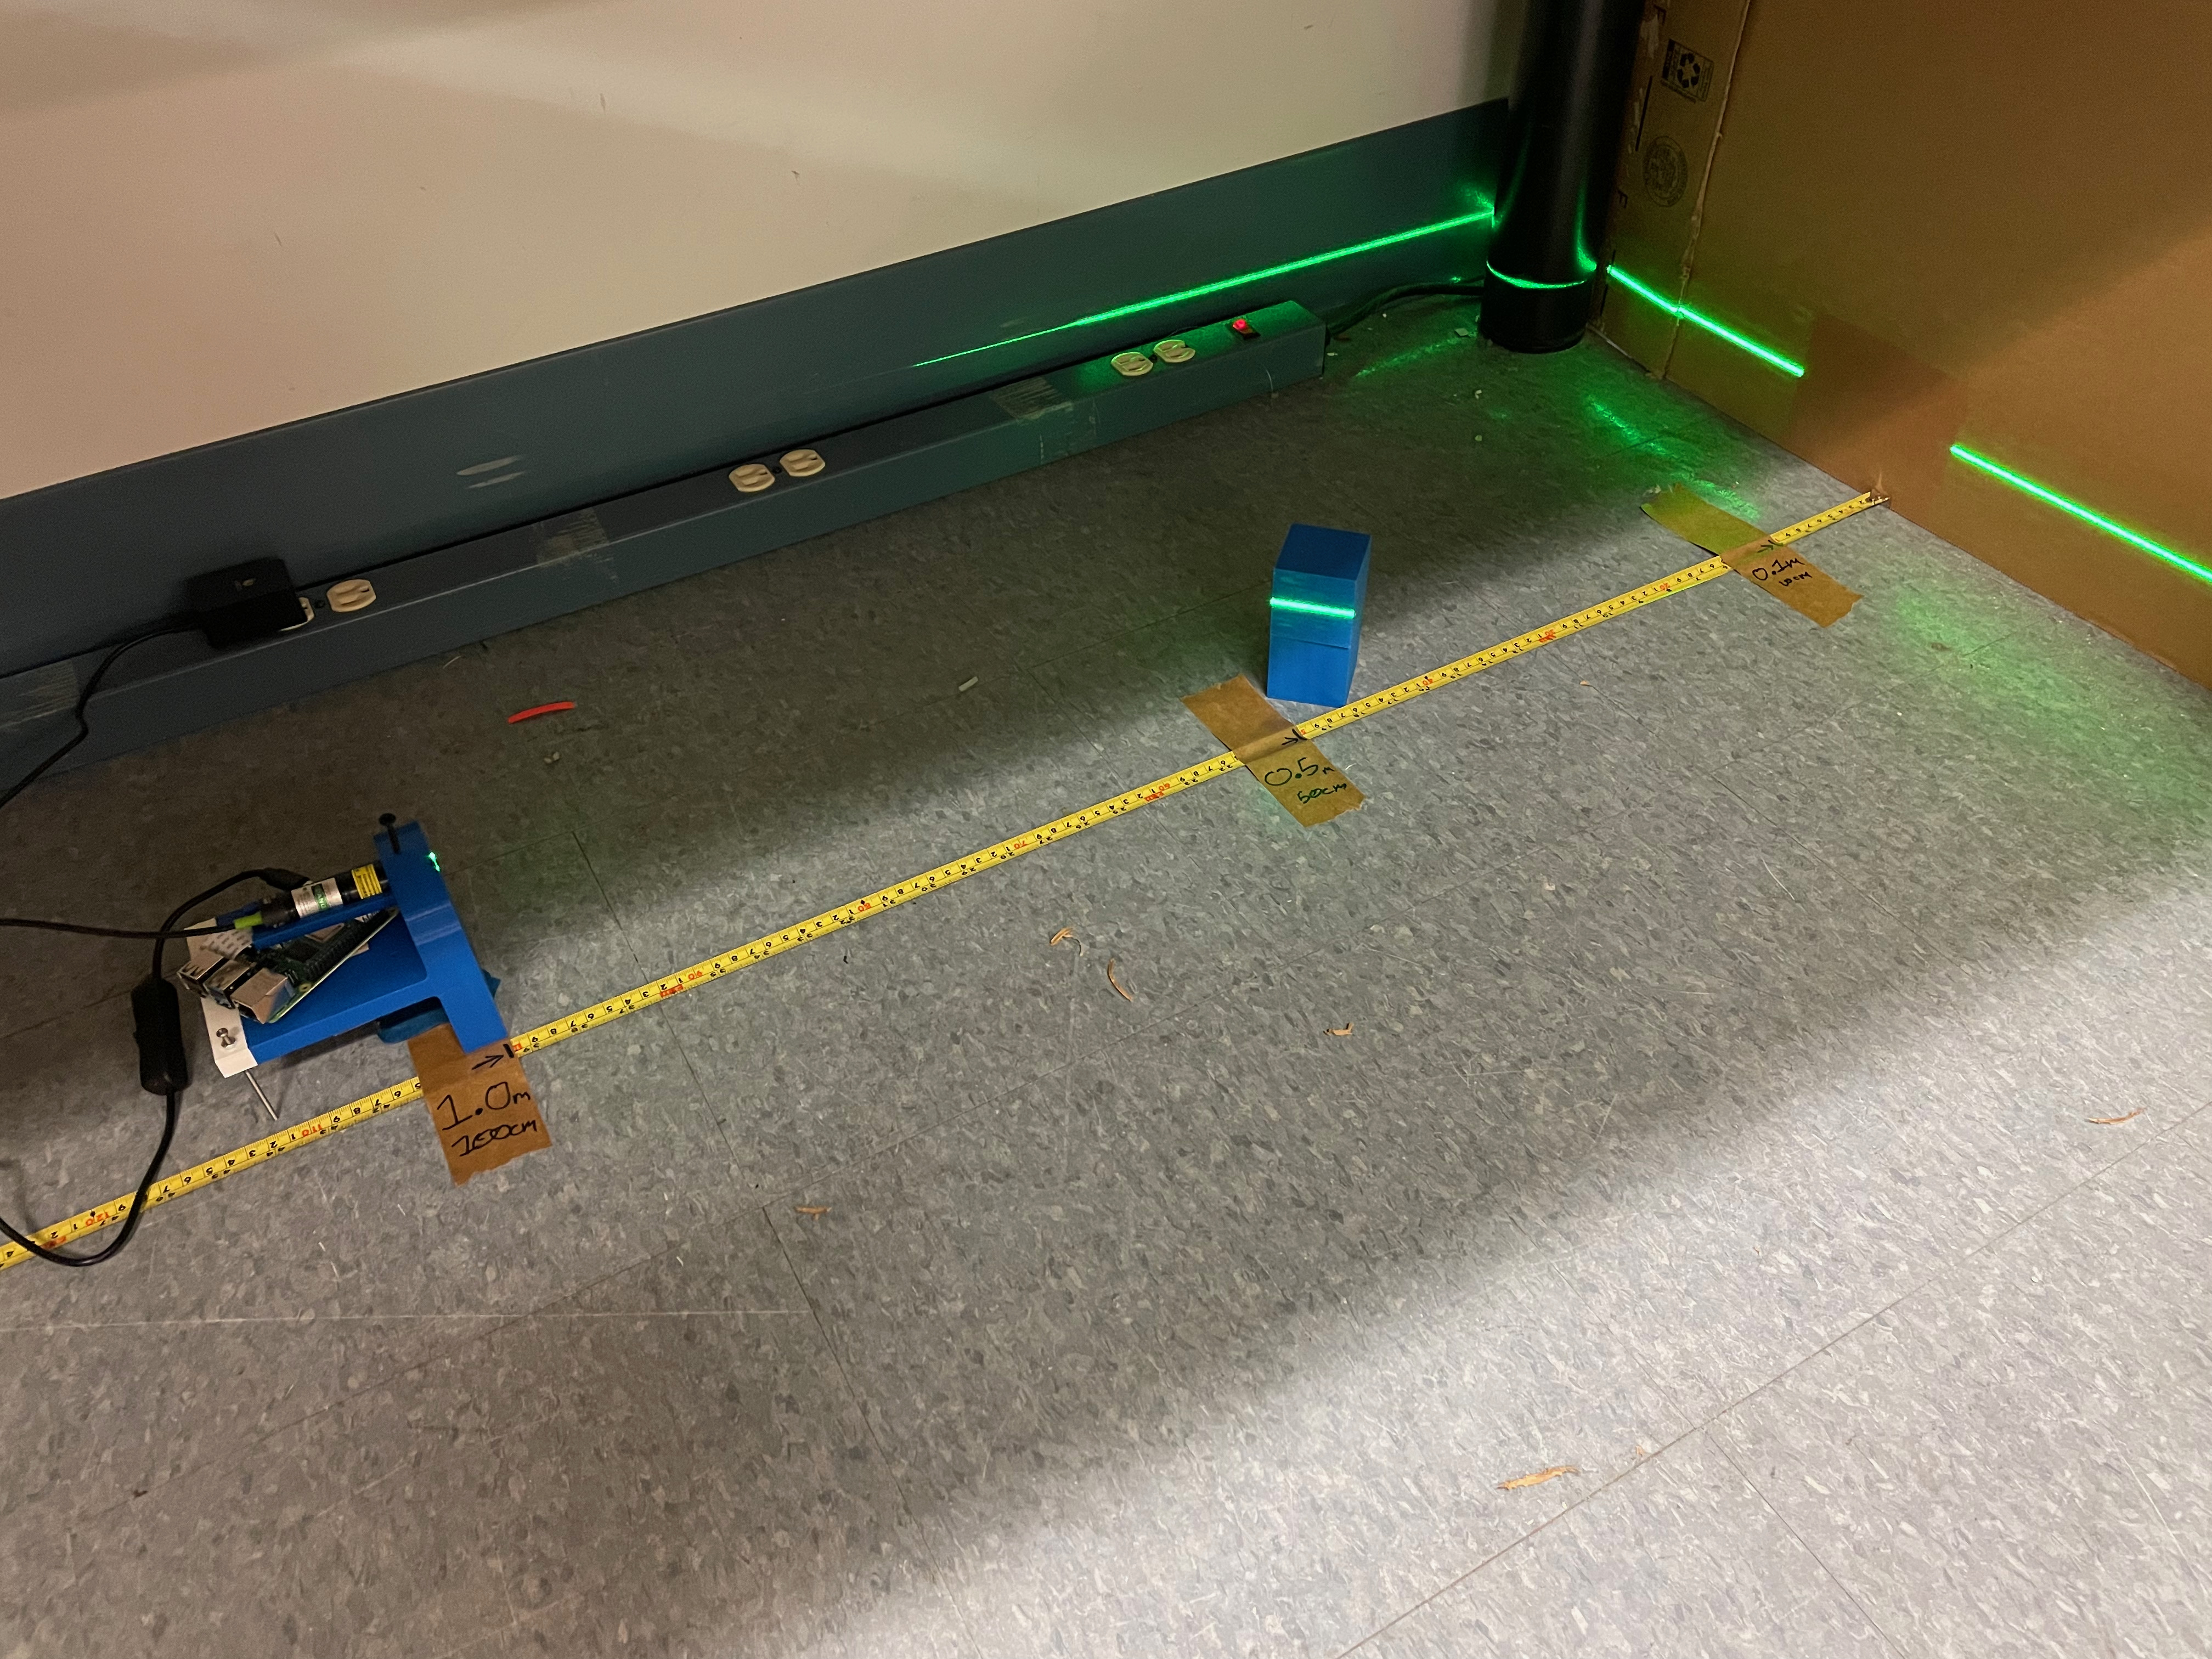
\includegraphics[width=0.8\linewidth]{laser-cave-inside.jpeg}
    	\caption{Inside}
    	\label{fig:laser-cave:inside}
    \end{subfigure}
	
	\caption{\smaller{The Laser Cave isolated testing environment, constructed from a table, cardboard, and duct-tape.}}
	
	\label{fig:laser-cave}
\end{figure}

\section{Results} \label{sec:results}

\subsection{Platform} \label{sec:results:platform}

The Raspberry Pi was a versatile and highly effective development platform, and I would endorse continuing to use it. The Raspberry Pi HQ Camera, however, ended up being rather difficult to properly focus (especially considering its labels are rather counter-intuitive). Especially considering our inability to source a C-Mount filter, evaluating simpler options for a camera might be worthwhile.

Additionally, MATLAB's Raspberry Pi integration leaves much to be desired. While it does make it easy to work with images, it's slow and buggy (in addition to MATLAB's general poor performance and instability, especially on macOS). In the future, investigating a middle ground between C++ and MATLAB (perhaps Python and OpenCV) would be worthwhile.

\subsection{Filtering \& Laser Detection} \label{sec:results:filtering-laser-detection}

The bandpass filter was highly effective at filtering out non-laser light, however reflections/glow from laser light often bounced against other surfaces and passed through the filter, thereby requiring additional processing (see \autoref{fig:image}). Several steps of additional processing were used (see \code{camera.m}):

\begin{itemize}
    \item MATLAB's camera calibration toolkit was used to account for and correct camera lens distortion.
    \item The image was rotated slightly to account for the laser beam being imperfectly horizontal (see \ref{sec:methods:hardware:optics-laser}). This correction was imperfect, and better aligning the laser would be a significant improvement.
    \item Only the green channel of the image was used, because the laser used was green.
    \item The image was thresholded, where each pixel was considered either \code{on} or \code{off}, depending on if its green value was greater than 75 (out of 255).
    \item For each column of pixels, the center position of the laser was calculated by finding the center of the largest block of continuous \code{on} pixels.
    \item Columns with zero \code{on} pixels were ignored.
\end{itemize}

\begin{figure} [!h]

	\centering
	
	\begin{subfigure}{.5\textwidth}
	    \centering
    	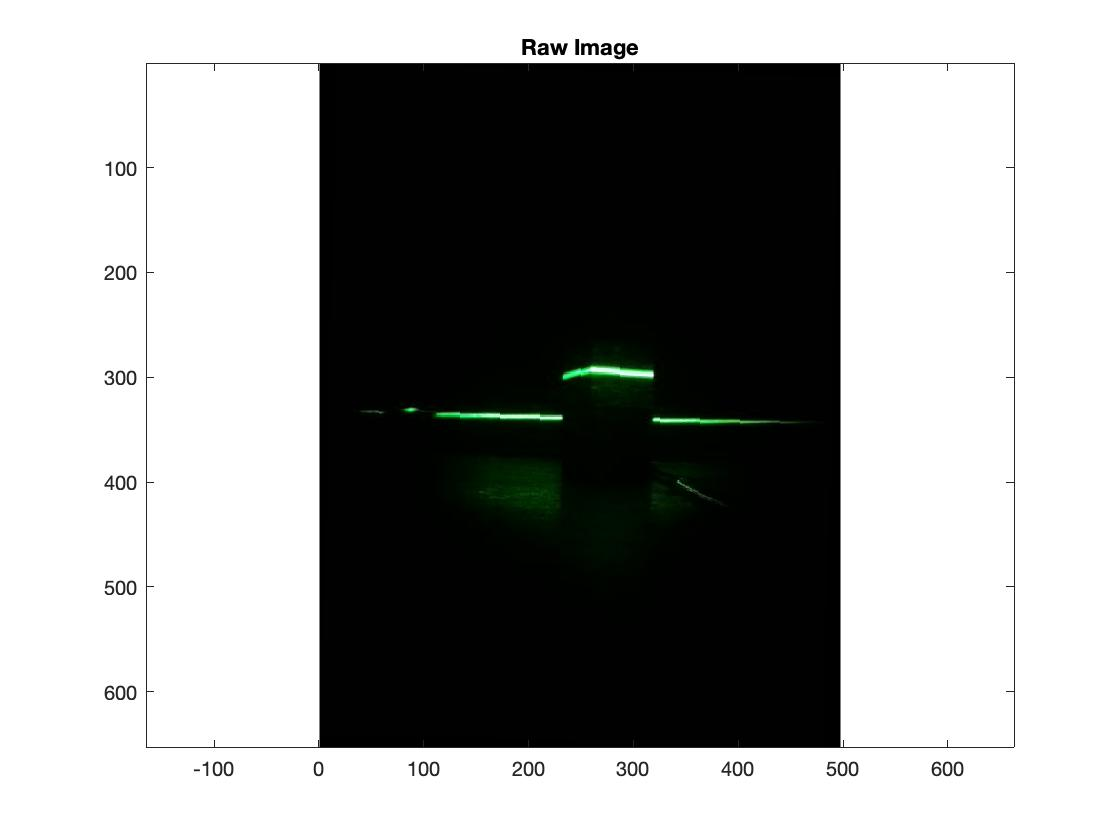
\includegraphics[width=1\linewidth]{camera-raw.jpg}
    	\caption{Raw (Post-Bandpass)}
    	\label{fig:image:raw}
    \end{subfigure}% <-- this comment is important to prevent a space
	\begin{subfigure}{.5\textwidth}
	    \centering
    	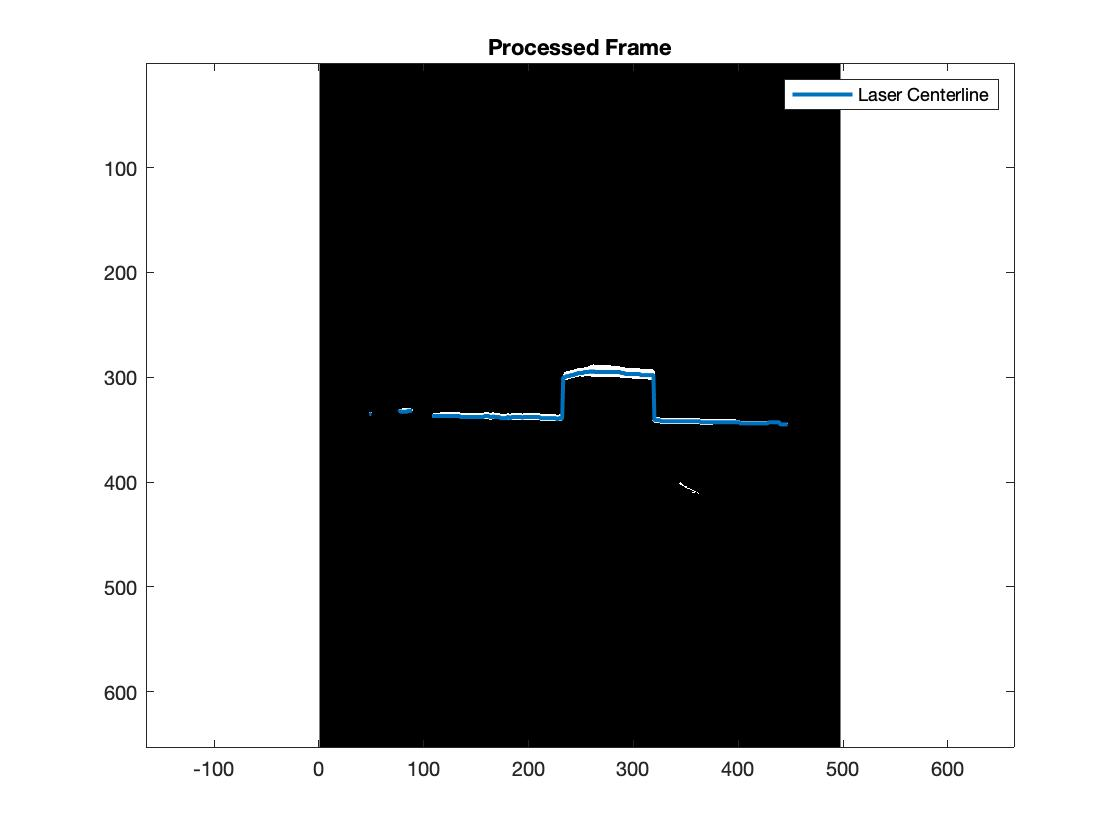
\includegraphics[width=1\linewidth]{camera-processed.jpg}
    	\caption{Processed}
    	\label{fig:image:processed}
    \end{subfigure}
	
	\caption{\smaller{Post-bandpass raw and fully-processed images of the laser. Reflection of laser light (in this case, off the ground) can be seen.}}
	
	\label{fig:image}
\end{figure}

\subsection{Distance Measurement} \label{sec:results:distance-measurement}

Once the center position of the laser was determined, it was translated into a set of distances from the camera (again, on a column-by-column basis) using \autoref{eqn:distance}, where $Y_0$ is the pixel row index where the laser beam intersects the center of the camera's vision, $\theta$ represents the angle between the laser and the horizontal (as calculated in CAD), and $\alpha$ represents an experimentally-determined constant roughly corresponding to half the distance between the center of the camera and the center of the laser, in pixels.

\begin{equation} \label{eqn:distance}
    \alpha\left(Y_0 - y\right)\arctan\left(\theta\right)
\end{equation}

$Y_0$ was calibrated by positioning the testbed 1 meter from the wall (the theoretical distance at which the laser beam and the camera's view intersect) and setting $Y_0$ to the pixel row index of the laser center line. $\alpha$ was determined (after calibrating $Y_0$) by moving the testbed to various distances from the wall and adjusting $\alpha$ to result in the most accurate results for all values. The system was then tested by placing it at as-yet-uncalibrated distances from the wall and comparing the calculated distance to the known distance.

This system was rather inaccurate, and needs substantial iteration (it's unclear if the algorithm is inaccurate, the calibration mechanism is inaccurate, or both). \cite{idrobo-pizo_calibration_2019} showed great promise in the area of calibration, but unfortunately I ran out of time to fully explore it.

\section{Conclusion} \label{sec:conclusion}

I developed the first stages of an underwater structured light profilometry system. At time of writing, the project is in the early prototype stage, where I built a simple testbed that holds the camera, laser, and supporting electronics. The prototype can accurately filter and detect laser light, however more research is needed into proper calibration. 

\section{Acknowledgements}

Thank you to Dave Barrett and the Olin RoboLab for making this research possible---I absolutely could not have accomplished this project without his support and guidance. Thank you also to all of my fellow researchers in the RoboLab, who have helped me countless times throughout this semester.

\medskip

\nocite{*}
\printbibliography

\end{document}
